%Removed by Marcella since we already hava a chapter involving MLP
\section{Artificial Neural Networks} \label{neuralnetsection}

Part of the theoretical basis underlying Deep Learning  initially emerged as models for understanding learning, that is, how the brain works. Thus, these theories became known as Neural Networks, one of the areas of Deep Learning  that has grown the most in recent years \cite{goodfellow2016}. Currently, the concepts of Neural Networks address more generic principles, not restricted to the perspective of neuroscience. Even though Neural Networks cannot explain much about the brain and cannot be suggested as realistic models of biological function, many aspects of learning still remain inspirational.

Networks were designed to acquire knowledge through a learning process. Similar to what happens in the brain, interactions between neurons, or synaptic weights, are responsible for storing knowledge. In practical terms, knowledge of a network would be the ability of a machine to autonomously perform complex functions, such as classifications and pattern recognition. Networks are also able to generalize learned information, extracting essential features from examples and guaranteeing coherent responses to new cases \cite{haykin1999}.

Even though the term Neural Network has only started to gain prominence in recent years, the first theoretical studies began around 1940 \cite{goodfellow2016}. One of the first published works was ``A Logical Calculus of the Ideas Immanent in Nervous Activity'' of 1943 \cite{mcculloch1943}, in which the authors, Warren McCulloch and Walter Pitts, presented an artificial model of a neuron from the theory of logical networks of nodes \cite{goodfellow2016}.

Figure \ref{fig:figure103} presents a simplification of a biological neuron, divided into three main parts: the cell body, dendrites, and axon. A neuron receives information, or nerve impulses, from the dendrites. This information is processed in the cell body and new impulses are transmitted through the axon to other neurons. The communication between neurons, the synapse, controls the transmission of impulses, determining the flow of information based on the strength of the received signal \cite{haykin1999}.

\begin{figure}
    \centering
    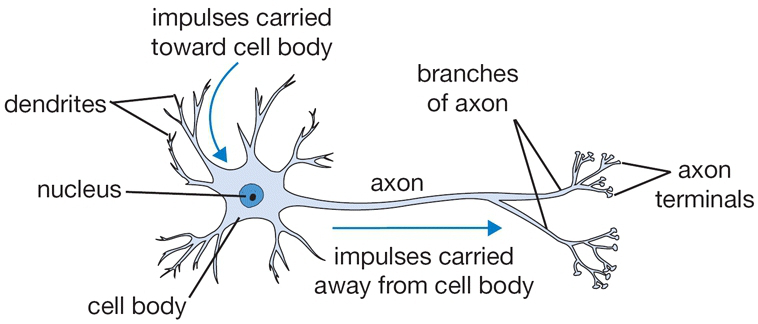
\includegraphics[scale=0.4]{"Part 3 - Learning Systems/Supervised Learning/Deep Learning/images/figure103.png"}
    \caption{Representation of a biological neuron \cite{img:neuronCS}.}
    \label{fig:figure103}
\end{figure}

By analogy to the previous paragraph, McCulloch and Pitts mathematically described an artificial neuron as a model with multiple input terminals $x_m$, representing the dendrites, and only one output point $y_k$, such as an axon Figure \ref{fig:figure104}. To simulate the behavior of synapses, each input $x_m$ is associated with a weight $w_{km}$, and the sum represents the received signal strength $v_k$.

\begin{figure}
    \centering
    \includegraphics[scale=0.7]{"Part 3 - Learning Systems/Supervised Learning/Deep Learning/images/figure104.png"}
    \caption{Mathematical representation of an artificial neuron.}
    \label{fig:figure104}
\end{figure}

The response signal is established by an activation function $\varphi$ applied to the weighted sum value. This function presents threshold behavior, Equation \ref{thresholdactivation}, in which the output is 1 or 0 according to the threshold value Figure \ref{fig:figure105}. The model can also include a bias $b_k$ in the summation to increase the degree of freedom of the activation function and ensure that a neuron does not have a null output even if the received signals are null. The bias value is adjusted along with synaptic weights \cite{haykin1999}.

\begin{equation}
\label{thresholdactivation}
y_k=\varphi(\upsilon_k)=
\begin{cases}
 1 \text{ if } \upsilon_k > 0 \\ 
 0 \text{ if } \upsilon_k \leq 0 
\end{cases}  
\end{equation}

\begin{figure}
    \centering
    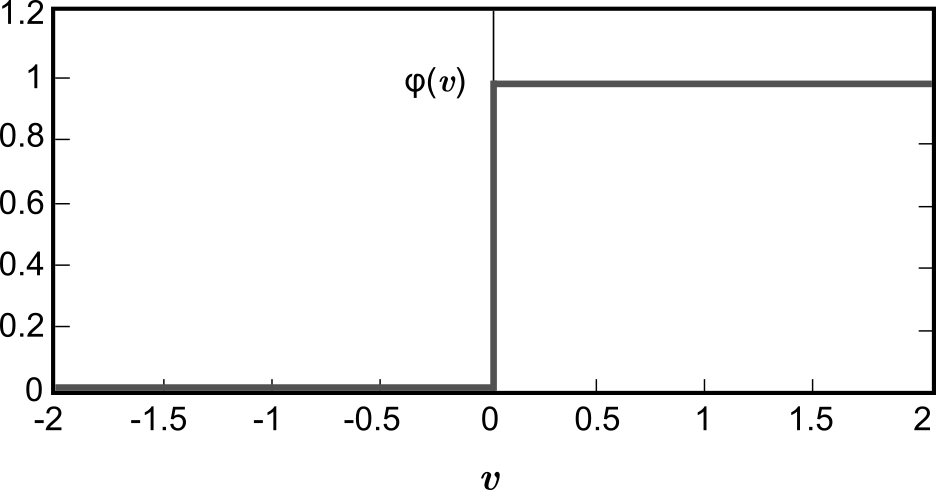
\includegraphics[scale=0.55]{"Part 3 - Learning Systems/Supervised Learning/Deep Learning/images/figure105.png"}
    \caption{Threshold Activation Function.}
    \label{fig:figure105}
\end{figure}

The model proposed by McCulloch and Walter Pitts could perform classifications in two categories. However, the weights needed to be adjusted manually as they did not have the ability to learn \cite{goodfellow2016}. One of the first discussions of learning rules in synaptic weight corrections was published in 1949 in Donald Hebb's book The Organization of Behavior \cite{haykin1999}. In Hebb's postulate, it is shown that the connection between neurons is strengthened each time it is used, thus, the neural pathways in the brain are continually modified and form clusters.

The first neural network capable of learning category weights was the Perceptron introduced by Frank Rosenblatt in 1958 \cite{haykin1999}. Perceptron had an architecture similar to Figure \ref{fig:figure106}, a single-layer network in addition to input and supervised learning. Initially, high expectations were raised about the possible applications of Perceptron, however, limitations soon began to be highlighted, many described in the book by Marvin Minsky and Seymour Papert published in 1969 \cite{minsky1969perceptrons}. One of the limitations is that the single-layer Perceptron performs only the classification of patterns that are linearly separable into two categories, which cannot, for example, represent the logic operator XOR, which is not linearly separable \cite{haykin1999}.


\begin{figure}
    \centering
    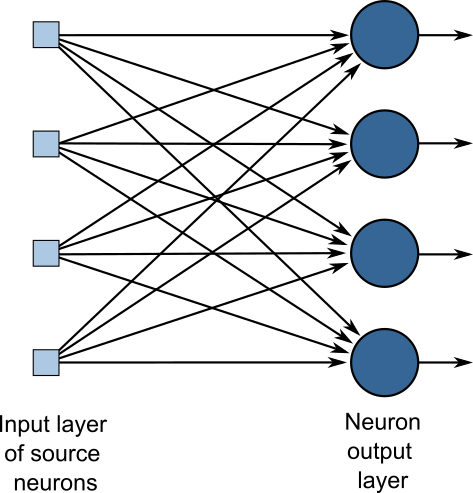
\includegraphics[scale=0.65]{"Part 3 - Learning Systems/Supervised Learning/Deep Learning/images/figure106.png"}
    \caption{One layer network architecture.}
    \label{fig:figure106}
\end{figure}

The negative image about Perceptron and its technological limitations diminished the popularity of neural networks, which reduced the number of researches in the area until the 1980s \cite{goodfellow2016}. Interest in neural networks began to increase, mainly due to the use of the distributed parallel processing approach, as applied to the backpropagation algorithm presented by Rumelhart, Hinton and Williams in 1986 \cite{rumelhart1986learning}. Backpropagation is the most widely used algorithm for Deep Learning  to date and was crucial to the training of MLP \cite{haykin1999}.

\section{MLP network}

For the multilayer Perceptron network to learn, it would be necessary to back-propagate the errors backwards between the layers, making possible the minimization of the cost function. The need to calculate the error derivative implied the appearance of activation functions different from those used in the original Perceptron model, without an abrupt activation, 0 or 1(Figure \ref{fig:figure105}) \cite{haykin1999}.  Considering that activation functions are one of the elements used to include nonlinearity, a key point for models not to be limited to linearly separable patterns, the approach was to incorporate nonlinear functions, but "well behaved" ones, that is, which are “almost” linear, continuous and derivable.

As the activation functions are responsible for the intermediation of responses between layers, nonlinear formats that do not radically alter the network response should be considered. The profiles that were closest to these behaviors are those of the sigmoid functions: the hyperbolic tangent and the logistic function \cite{rateke1999}.

The sigmoid function has an S-shape, where at the ends the function has a constant behavior, which is evident in the graph of the logistic function (Figure \ref{fig:figure107}). The parameter $a$ of the logistic equation(Equation \ref{eq:logistic}), allows to parameterize the behavior of the function, changing the slope. The higher the value of $a$, the more the sigmoid function approaches the threshold function, Figure \ref{fig:figure105}.

\begin{figure}
    \centering
    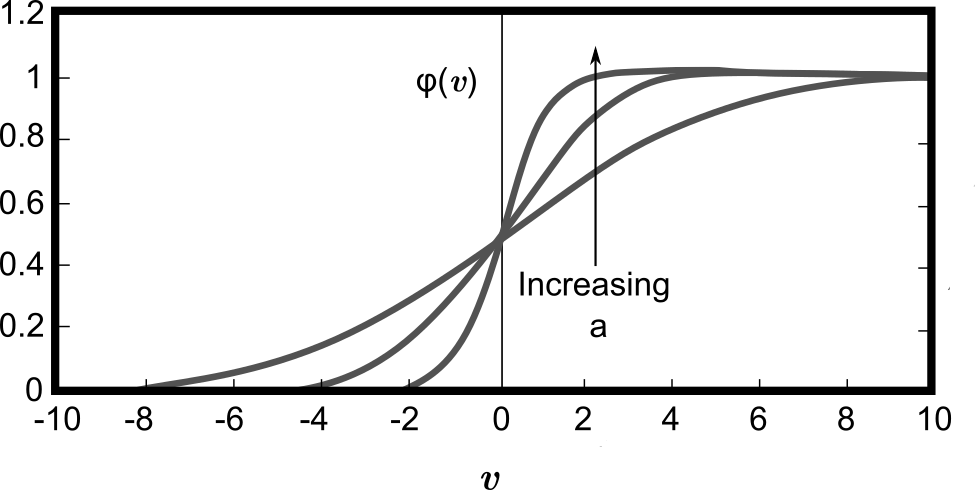
\includegraphics[scale=0.55]{"Part 3 - Learning Systems/Supervised Learning/Deep Learning/images/figure107.png"}
    \caption{Sigmoid function.}
    \label{fig:figure107}
\end{figure}

\begin{equation}
\label{eq:logistic}
\varphi(\upsilon)=
 \frac{1}{1+exp(-a)}
\end{equation}

Unlike the threshold function that takes values 0 or 1, the logistic function has results in a continuous interval between 0 and 1 \cite{haykin1999}. The sigmoid function is also differentiable, whereas the threshold function is not. An antisymmetric form of the sigmoid is the hyperbolic tangent function (Equation \ref{tanh}). The hyperbolic tangent function is defined in the interval [$-$1,1], which allows the sigmoid function to assume negative values as well \cite{haykin1999}.

\begin{equation}
\label{tanh}
\varphi(v)=tanh(av)
\end{equation}


When proposing an efficient method for training multilayer Perceptrons, it became interesting to include one or more layers of hidden neurons between the input and output layers. The combination of more layers allowed the network to be implemented for more complex problems, not restricted to the linear transformations of the original Perceptron model. Through hidden layers, it is possible to progressively extract important characteristics that define input patterns \cite{haykin1999}.

The initially proposed mathematical neuron was extended to a structure of processing elements connections, the network nodes. The elements were organized in layers, and different connection configurations were proposed. The most popular formats are defined as a neural network architecture, recognized by the number of layers in the network, number of nodes in each layer, and type of connection between nodes.

The MLP network architecture is composed of an input layer that receives the signal, an output layer that returns the result, and between them an arbitrary number of hidden layers (Figure \ref{fig:figure108}). Generally, choosing the number of nodes in the input and output layer is straightforward. For example, in an application with images, the number of neurons in the input layer could correspond to the number of pixels in the image and the output layer could be just a single neuron indicating the probability of actually being what you are looking for, the chance of a positive result. The arrangement of the intermediate layers is not so simple, however, it is often defined empirically based on the characteristics of the input data and the complexity of the problem \cite{braga1998fundamentos}.

\begin{figure}
    \centering
    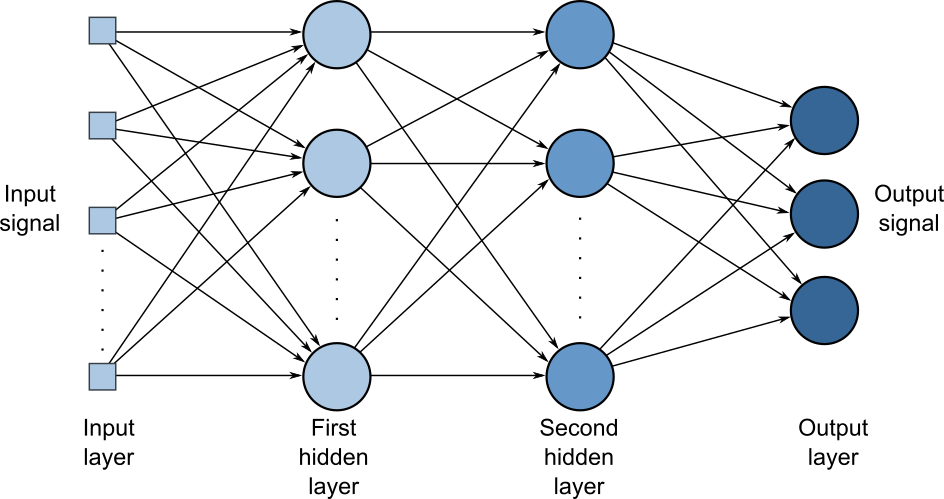
\includegraphics[scale=0.65]{"Part 3 - Learning Systems/Supervised Learning/Deep Learning/images/figure108.png"}
    \caption{MLP network architecture.}
    \label{fig:figure108}
\end{figure}

A common classification of architectures is based on the pattern of connections, two main classes being identified: direct networks (feedforward) and recurrent networks (feedback) \cite{haykin1999}. The MLP model has a feedforward type architecture, in which information propagation occurs in a single direction and nodes of the same layer are not connected to each other. The output from one layer is used as input to the next, with no loopings, that is, they are not sent back \cite{haykin1999}.
In the recurrent typologies, a feedback process occurs, in which the outputs of nodes are reinserted as inputs in previous nodes (Figure \ref{fig:figure109}). The behavior of the cycles is dynamic controlled by unit delays \cite{haykin1999}. The idea of the model is to stimulate signals in cascade effect with time dependence.

\begin{figure}
    \centering
    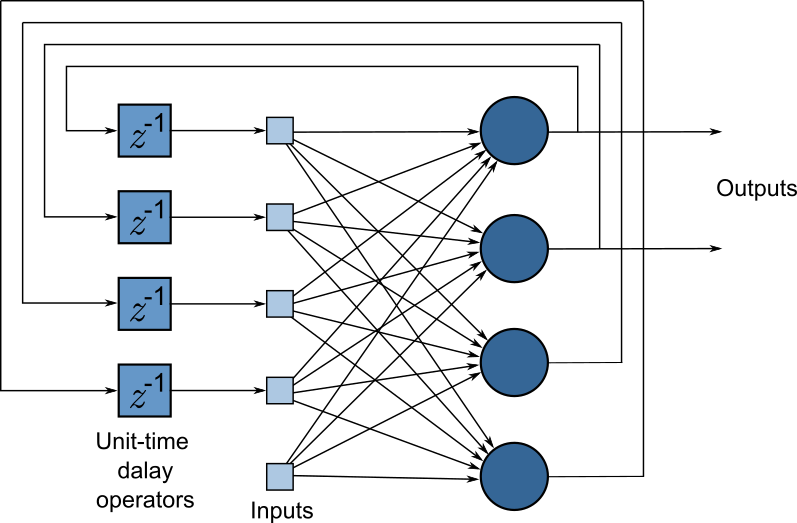
\includegraphics[scale=0.65]{"Part 3 - Learning Systems/Supervised Learning/Deep Learning/images/figure109.png"}
    \caption{recurrent network architecture \cite{haykin1999}}
    \label{fig:figure109}
\end{figure}

\section{Backpropagation}\label{backpropagation}

To explain the backpropagation algorithm in training neural networks, we will use an example of an MLP network application for number recognition. The Network Code\footnote{https://github.com/mnielsen/neural-networks-and-deep-learning} is an implementation of the online book “Neural Networks and Deep Learning” written by Michael Nielsen \cite{nielsen2015}. The training data was taken from the MNIST dataset, which contains over 60,000 scanned images of numbers written along with classification labels. The information was collected by the National Institute of Standards and Technology of the United States (NIST), and the images are in grayscale and pixel size of 28x28 as in Figure \ref{fig:figure110}.

\begin{figure}
    \centering
    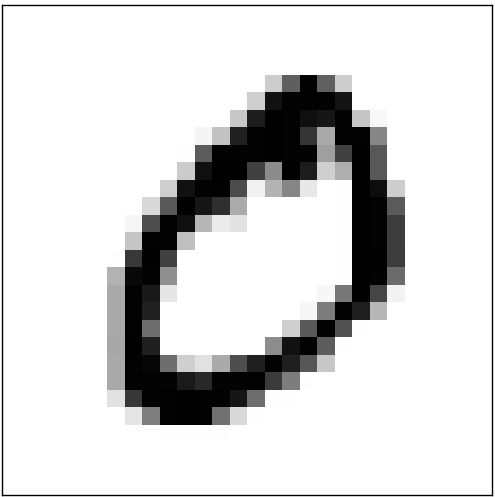
\includegraphics[scale=0.5]{"Part 3 - Learning Systems/Supervised Learning/Deep Learning/images/figure110.png"}
    \caption{An example of number zero selected from the MNIST dataset.}
    \label{fig:figure110}
\end{figure}

The original MNIST dataset is divided into two parts, one containing 60,000 images for training and the other containing 10,000 images for the testing phase, in which the accuracy of the network trained to recognize digits is evaluated. In the example of author Michael Nielsen, the original training data were also reorganized into two groups, the first with 50,000 images that were used in the training and the other part, 10,000 images, which was reserved for the validation in which the hyperparameters of the network.

Considering 28x28 pixel images, the input data was defined as vector $x$ of dimension 784, where each position corresponds to a pixel value of the image. For the output vector $y$ of the network, the dimension 10 was established, in which each position refers to a digit of 0 to 9. Thus, if an input matches the number 3 then the expected output will be the vector transposed in the form $y(x)=(0,0,0,1,0,0,0,0,0,0)^T$. Based on the format of the input and output data from the network, the example was built with a three-layer MLP network as in Figure \ref{fig:figure111}, with the first layer having 784 nodes and the last layer having 10 nodes. In the middle layer, the hidden layer, we will use 30 nodes, but it is worth noting that author Michael Nielsen defined the number of nodes after some tests, optimizing the choice of network parameters.

\begin{figure}
    \centering
    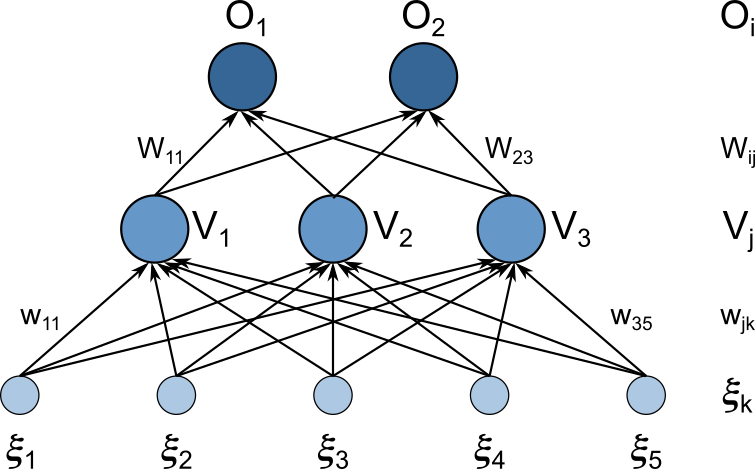
\includegraphics[scale=0.55]{"Part 3 - Learning Systems/Supervised Learning/Deep Learning/images/figure111.png"}
    \caption{MLP network with a hidden layer.}
    \label{fig:figure111}
\end{figure}

The data are taken from the zip file “mnist.pkl.gz”, subdivided into training, validation and testing, and then configured in the proposed network format.

At the Algorithm \ref{lst:classnetwork}, the network is constructed from the command “Network([784, 30, 10], cost=QuadraticCost)”, where each argument corresponds to the number of nodes in the layer. The attributes of the “Network” class include the number of layers “num\_layers,” the number of nodes in each layer “sizes,” the initial weights and bias, which are randomly generated by the “default\_weight\_initializer(),” method, and the cost function “ cost.” The cost function applied in this example is defined in the QuadraticCost class, and the quadratic error (Mean Squared Error - MSE) was used.

\begin{lstlisting}[caption={Delta method in Python},label={lst:classnetwork},language=Python]
class Network(object):
  def __init__(self, sizes, cost=QuadraticCost):
    self.num_layers = len(sizes)
    self.sizes = sizes
    self.default_weight_initializer()
    self.cost=cost
\end{lstlisting}

Next, we will present a summary of the mathematical theory of the backpropagation method and to facilitate this process we will use the nomenclature of the elements of a neural network based on the book “Introduction To The Theory Of Neural Computation” \cite{hertz2018}. In the training of a network like the one in Figure \ref{fig:figure111}, a training set is presented as $\{\xi_k^\mu,\zeta_i^\mu\}$, in which each pattern presented $(\mu=1,2,\dots,p)$ corresponds to a pair: input $(\xi_k^\mu)$ and expected output $(\zeta_i^\mu)$. In this example, the number of patterns in training is $p=50000$. The index $k$ in the input layer references the value at each node of the layer, and the index $i$ to the nodes of the output layer. The final response from the network is labeled $O_i$ and the hidden layer output signal is $V_j$. The connection between the input layer and the hidden layer is established by the weights $w_{jk}$, and the weights $W_{ij}$ connect the output layer with the middle one.

Backpropagation is a supervised method in which training takes place in two phases \cite{haykin1999}. In the forward step, an input is presented to the network and, according to the connections established between the layers, the response signals are successively propagated to the output layer, generating a result that is expected to be the closest to the standard. Each node of a subsequent layer connects with all nodes of the previous layer, and the signal received by this node is a weighting of the weights of all connections. The input signal from each node is biased and passed to the next layer as a response to an activation function $g$. The output response of a node will be called $V_j$ if the signal goes to an intermediate layer, or $O_i$ if it is directed to the output layer.

Imagine that a node $j$ in the middle layer receives as input:

\begin{equation}
\label{xisum1}
h_j^\mu=\sum_{k}w_{jk}\xi_k^\mu
\end{equation}

And produces in response:
\begin{equation}
\label{vequal}
V_j^\mu=g(h_j^\mu)=g(\sum_kw_{jk}\xi_k^\mu)
\end{equation}

Thus, a node in the output layer receives the propagated signal as input:
\begin{equation}
\label{sumsums}
h_i^\mu=\sum_kW_{ij}V_j^\mu=\sum_kW_{ij}g(\sum_kw_{jk}\xi_k^\mu)
\end{equation}

generating as a response from the output of the network:
\begin{equation}
\label{outeq}
O_i^\mu=g(h_i^\mu)=g(\sum_kW_{ij}V_j^\mu)=g(\sum_kW_{ij}g(\sum_kw_{jk}\xi_k^\mu))
\end{equation}

At the Algorithm \ref{lst:feedforward}, the forward phase is represented by the following method:

\begin{lstlisting}[caption={Delta method in Python},label={lst:feedforward},language=Python]
feedforward(self, a):
  for b, w in zip(self.biases, self.weights):
    a = sigmoid(np.dot(w, a)+b)
  return a
\end{lstlisting}

At the Algorithm \ref{lst:sigmoid}, the activation function is the logistic function defined by the “sigmoid()” method and its derivative is calculated in the “sigmoid\_prime()” method.

\begin{lstlisting}[caption={Delta method in Python},label={lst:sigmoid},language=Python]
sigmoid(z):
  return 1.0/(1.0+np.exp(-z))
 
sigmoid_prime(z):
  return sigmoid(z)*(1-sigmoid(z))
\end{lstlisting}

In the second phase, backward, the weights and bias are corrected layer by layer, from the network's output to its input, in an iterative process so that the output $O_i$ is closer and closer to the expected pattern $\zeta_i$, reducing the error \cite{haykin1999}. One way to assess how the error is reduced in relation to parameter changes is to determine an error function, or cost, dependent on weights and bias. According to Equation \ref{mserror}, we adopt the mean squared error (MSE) as a cost function.

\begin{equation}
\label{mserror}
E[w]=\frac{1}{2}\sum_{\mu i}[\zeta_i^\mu-O_i^\mu]^2 = \frac{1}{2}[\zeta_i^\mu - g(\sum_kW_{ij}g(\sum_kw_{jk}\xi_k^\mu))]^2
\end{equation}
At the Algorithm \ref{lst:fn}, the cost function (MSE) is presented in the “fn()” method in the “QuadraticCost” class:

\begin{lstlisting}[caption={Delta method in Python},label={lst:fn},language=Python]
fn(a, y):
  return 0.5*np.linalg.norm(a-y)**2
\end{lstlisting}



Error reduction involves an optimization process, called gradient descent, which seeks to determine the parameters (weights and bias) that minimize the cost function \cite{nielsen2015}. In this method, the error variation can be written as partial derivatives of the error as a function of the weights, composing the error gradient vector. As the gradient vector points towards the greatest increase in error, the variation in weights is given by the negative gradient, ensuring a faster error reduction. Thus, according to Equation \ref{minimizeError}, the descending gradient rule applied to the connections between the hidden and output layer can be written as:

\begin{equation}
\label{minimizeError}
\Delta W_{ij}=-\eta\frac{\partial E}{\partial W_{ij}}=\eta\sum_\mu[\zeta_i^\mu-O_i^\mu]g'(h_i^\mu)V_j^\mu=\eta\sum_\mu\delta_i^\mu V
\end{equation}

\begin{equation*}
\delta_i^\mu=[\zeta_i^\mu-O_i^\mu]g'(h_i^\mu)
\end{equation*}

The weight modification formula is known as the delta rule and receives the term $\eta$, the learning rate, to promote a gradual correction, without sudden changes \cite{nielsen2015}. The term $g'$ refers to the derivative of the activation function and appears in the formula due to the derivation of the error function. The delta rule applied in the connections between the hidden and the input layer uses the chain rule because the derivatives are in relation to the weights $w_{jk}$, which are presented as a more implicit dependence on the error. The correction of weights can be represented by Equation \ref{correcaoPesos}:

\begin{equation}
\begin{split}
\Delta w_{ij}&=-\eta\frac{\partial E}{\partial w_{jk}}\\&=-\eta\sum_\mu\frac{\partial E}{\partial V_j^\mu}\frac{\partial V_j^\mu}{\partial w_{jk}}\\&=\eta\sum_{\mu i}[\zeta_i^\mu-O_i^\mu]g'(h_i^\mu)W_{ij}g'(h_j^\mu)\xi_k^\mu
\\&=\eta\sum_{\mu i}\delta_i^\mu W_{ij}g'(h_j^\mu)\xi_k^\mu=\eta\sum_\mu\delta_j^\mu\xi_k^\mu
\end{split}
\label{correcaoPesos}
\end{equation}

\begin{equation*}
\delta_j^\mu=g'(h_j^\mu)\sum_i\delta_i^\mu W_{ij}
\end{equation*}

This rule can also be extended to networks with more than one hidden layer \cite{rateke1999}. The generalized delta rule for the m-th layer of a network can be described by Equation 1.13:

\begin{equation}
\Delta w_{pq}^m=\eta\sum_\mu\delta_p^{m,\mu}V_q^{m-1,\mu}
\end{equation}

\begin{equation}
\delta_p^{m, \mu} =
  \begin{cases}
    \text{if m is the Output layer, } &[\zeta_p^\mu-O_p^\mu]g'(h_p^{m,\mu})\\
    \text{otherwise, } &g'(h_p^{m,\mu})\sum_r\delta_r^{m+1,\mu}w_{rp}^{m+1}
  \end{cases}
\end{equation}

The correction of weights takes place considering the connections between each two layers, one closer to the output ($p$) and the other more internal ($q$). The vector $V_q$ represents the activation signal received by the layer of nodes “$p$”, and when the calculation involves the input layer and the first hidden layer this vector is the input pattern ($\xi_k^\mu$). The delta factor ($\delta$) works as a memory of the responses of the outermost layers, that is, to modify the weights backwards, it is necessary that the layer connections keep memory of the layers that were changed previously. The backpropagation algorithm is used in the training step, through the "backprop()" method in Algorithm \ref{lst:backprop}:

\begin{lstlisting}[caption={Backpropagation method in Python},label={lst:backprop},language=Python]
backprop(self, x, y):
    nabla_b = [np.zeros(b.shape) for b in self.biases]
    nabla_w = [np.zeros(w.shape) for w in self.weights]
    # feedforward
    activation = x
    activations = [x] 
    zs = [] 
    for b, w in zip(self.biases, self.weights):
        z = np.dot(w, activation)+b
        zs.append(z)
        activation = sigmoid(z)
        activations.append(activation)
    # backward pass
    delta = (self.cost).delta(zs[-1], activations[-1], y)
    nabla_b[-1] = delta
    nabla_w[-1] = np.dot(delta, activations[-2].transpose())
    for l in range(2, self.num_layers):
        z = zs[-l]
        sp = sigmoid_prime(z)
        delta = np.dot(self.weights[-l+1].transpose(),delta) * sp
        nabla_b[-l] = delta
        nabla_w[-l] = np.dot(delta, activations[-l-1].transpose())
    return (nabla_b, nabla_w)
\end{lstlisting}

As highlighted earlier, the first phase of backpropagation is feedforward. In this step, an input pattern ($x$) is received and the weights and bias randomly initialized. After the sum of the weights and bias weights between two layers, this value is saved in the vector “zs[ ],” and the result of activating this value is saved in “activations[ ].” The next layer input is the activation signal saved in “actvivation.” This process takes place from the input to the output layer, saving the activation signals from the hidden layers ($V_j$) in “activations[ ]”. In the backward pass phase, the delta($\delta$) is first calculated from the output layer response saved as the last element of the “activations[ ]” vector and the expected output pattern($y$). The delta value, in this case, is calculated from the “delta()” method of the “QuadraticCost” class as the product between the difference of the network output response ($a$) and the expected value ($y$) with the derivative of last layer activation signal as seen in Algorithm \ref{lst:delta}:

\begin{lstlisting}[caption={Delta method in Python},label={lst:delta},language=Python]
delta(z, a, y):
  return (a-y) * sigmoid_prime(z)
\end{lstlisting}

After calculating the first delta, the increment of weights ($\Delta W_{ij}$) between the last layer and the hidden layer is determined as the product of the delta ($\delta_i$) by the activation vector ($V_j$) that the last layer received as input. Weight increments are saved in the vector “nabla\_w[ ].” The deltas and weights increments of the hidden layer are obtained iteratively in the repetition structure. The calculation of the delta of the $m$ layer depends on the sum of the products of the delta calculated previously, of the outermost layer, with the weight vector of the $m$ layer. The summation value is multiplied by the derivative of the activation signal in the layer m. Then, the value of the increment of weights is obtained by the product of the current delta with the activation value received by layer $m$. After performing this same process for all layers, the function returns a vector with weight increments based on a pattern ($\xi_k^\mu,\zeta_i^\mu$), which occurs for all training patterns.

To speed up the learning process, instead of updating the weights each time a pattern is presented, author Michael Nielsen\cite{nielsen2015} suggests in his example the use of the stochastic gradient descending method. The idea is to randomly group the input patterns into what he calls a "mini-batch." In the update\_mini\_batch() method, the backprop function returns the calculated weight increment for each pattern within the batch, and these are summed in nabla-w until the entire batch is presented, and then the weights and bias are adjusted. Then the other “mini-batch” are presented until the entire training set is used, ending a training season. That is, at each time, the training set is subdivided into batches, and the weights are updated only at the end of each batch presentation as shown in Algorithm \ref{lst:batch}:

\begin{lstlisting}[caption={update\_mini\_batch() method in Python},label={lst:batch},language=Python]
update_mini_batch(self, mini_batch, eta, lmbda, n):
    nabla_b = [np.zeros(b.shape) for b in self.biases]
    nabla_w = [np.zeros(w.shape) for w in self.weights]
    for x, y in mini_batch:
        delta_nabla_b, delta_nabla_w = self.backprop(x, y)
        nabla_b = [nb+dnb for nb, dnb in zip(nabla_b, 
                delta_nabla_b)]
        nabla_w = [nw+dnw for nw, dnw in zip(nabla_w, 
                delta_nabla_w)]
    self.weights = [(1-eta*(lmbda/n))*w-(eta/len(mini_batch))*nw
                for w, nw in zip(self.weights, nabla_w)]
    self.biases = [b-(eta/len(mini_batch))*nb
                for b, nb in zip(self.biases, nabla_b)]
\end{lstlisting}

The training takes place using the “SGD()” method, which stands for descent of the stochastic gradient, in which the training set, the number of epochs, the size of the “mini\_batch\_size” grouping and the learning rate are passed as parameters.

\begin{lstlisting}[caption={SGD call in Python},label={lst:sgd},language=Python]
net.SGD(training_data,30,10,0.5, evaluation_data=test_data,
        monitor_evaluation_cost=True, monitor_evaluation_accuracy=True,
        monitor_training_accuracy=True, monitor_training_cost=True)
\end{lstlisting}

It's in the “SGD()” method”(Algorithm \ref{lst:SGD}), which occurs the subdivision of training patterns into "mini\_batch." Then, the “update\_mini\_batch()” function is called for each grouping until one epoch ends, and this is repeated for all epochs.

\begin{lstlisting}[caption={SGD method in Python},label={lst:SGD},language=Python]
SGD(self, training_data, epochs, mini_batch_size, eta,
    lmbda = 0.0, evaluation_data=None, 
    monitor_evaluation_cost=False, 
    monitor_evaluation_accuracy=False,
    monitor_training_cost=False, 
    monitor_training_accuracy=False):
  for j in range(epochs):
    random.shuffle(training_data)
    mini_batches = [training_data[k:k+mini_batch_size] 
                for k in range(0, n, mini_batch_size)]
    for mini_batch in mini_batches:
        self.update_mini_batch(mini_batch, eta, lmbda,
                                len(training_data))
    print ("Epoch %s training complete" % j)
\end{lstlisting}

Within the “SGD()” method it is possible to configure to evaluate the total error and accuracy of the network after each training period, considering both the training data and the test or validation data. To select the test data, they must be passed as parameters in “evaluation\_data”. When selecting the options “monitor\_evaluation\_cost” or “monitor\_training\_cost” the method “total\_cost()” is called(Algorithm \ref{lst:cost}) which returns the sum of the evaluated errors for the entire dataset.

\begin{lstlisting}[caption={total\_cost() method in Python},label={lst:cost},language=Python]
total_cost(self, data, lmbda, convert=False):
    cost = 0.0
    for x, y in data:
        a = self.feedforward(x)
        if convert: y = vectorized_result(y)
        cost += self.cost.fn(a, y)/len(data)
    return cost
\end{lstlisting}

After each epoch, a set of weights and bias is established, and when using the “feedforward()” method, these parameters define the output response of the network ($a$) for each input pattern ($x$). By comparing the answer ($a$) with the expected value ($y$) within the MSE cost function, method “fn()” of the class “QuadraticCost,” the error for each pattern is quantified. The “accuracy()” method in Algorithm \ref{lst:accuracy}, is used inside the “SGD()” when setting “monitor\_evaluation\_accuracy= True” or “monitor\_training\_accuracy= True.” This function returns the sum of results where the net output values matched the expected value ($y$). The network signal is calculated by the “feedforward()” function, which is used for each value ($x$) of the dataset, whether training or evaluation.

\begin{lstlisting}[caption={accuracy() method in Python},label={lst:accuracy},language=Python]
accuracy(self, data, convert=False):
    results = [(np.argmax(self.feedforward(x)), y) 
                for (x, y) in data]
    return sum(int(x == y) for (x, y) in results)
\end{lstlisting}

Considering that the values of the total error and the accuracy are calculated for each epoch, the training method “SGD()” returns four vectors inside a tuple(in Algorithm \ref{lst:return}), each one with the number of positions corresponding to the total number of epochs. Thus, if the training takes place in 30 epochs, then the first list in the tuple will have 30 elements corresponding to the total cost of the evaluation data at the end of each epoch.

\begin{lstlisting}[caption={Delta method in Python},label={lst:return},language=Python]
return evaluation_cost, evaluation_accuracy,
            training_cost,training_accuracy
\end{lstlisting}

Saved results can be plotted on graphs to visually assess network performance. A very common graph to monitor network training is the training cost, mainly because learning is guided by minimizing this curve. In Figure \ref{fig:figure113}, the cost curve for a configuration that uses the total training set (50000 images) and with 30 epochs is presented. However, it is not recommended to have only this graph as a basis to establish the network's hyperparameters, such as the learning rate and the number of training epochs. For example, Figure \ref{fig:figure114} also refers to a cost function, but for another training setup, which uses only 1000 training images and 100 epochs.

\begin{figure}
    \centering
    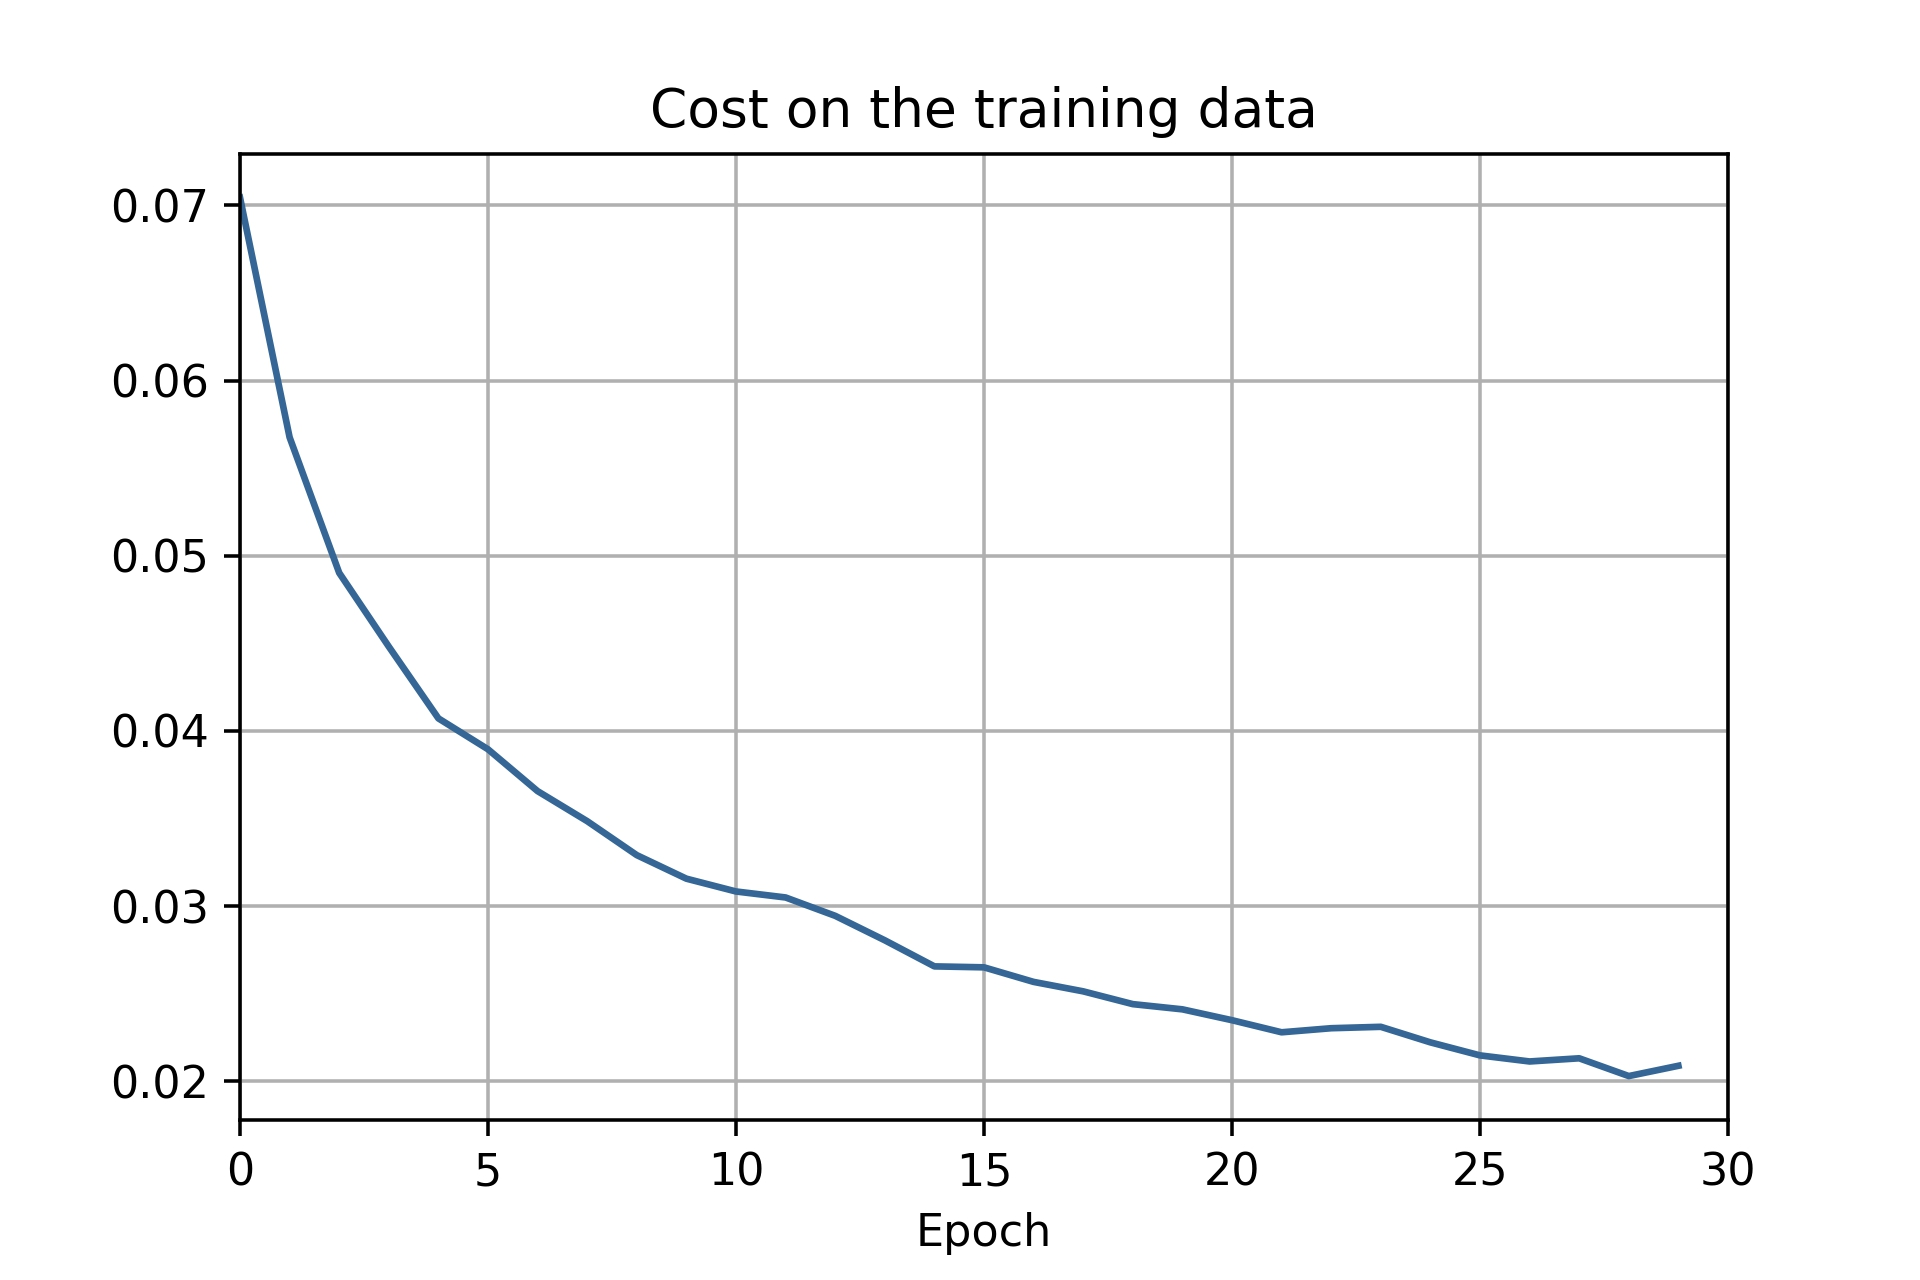
\includegraphics[scale=0.6]{"Part 3 - Learning Systems/Supervised Learning/Deep Learning/images/figure113.jpg"}
    \caption{Cost curve in training with 30 epochs and 50000 images.}
    \label{fig:figure113}
\end{figure}

\begin{figure}
    \centering
    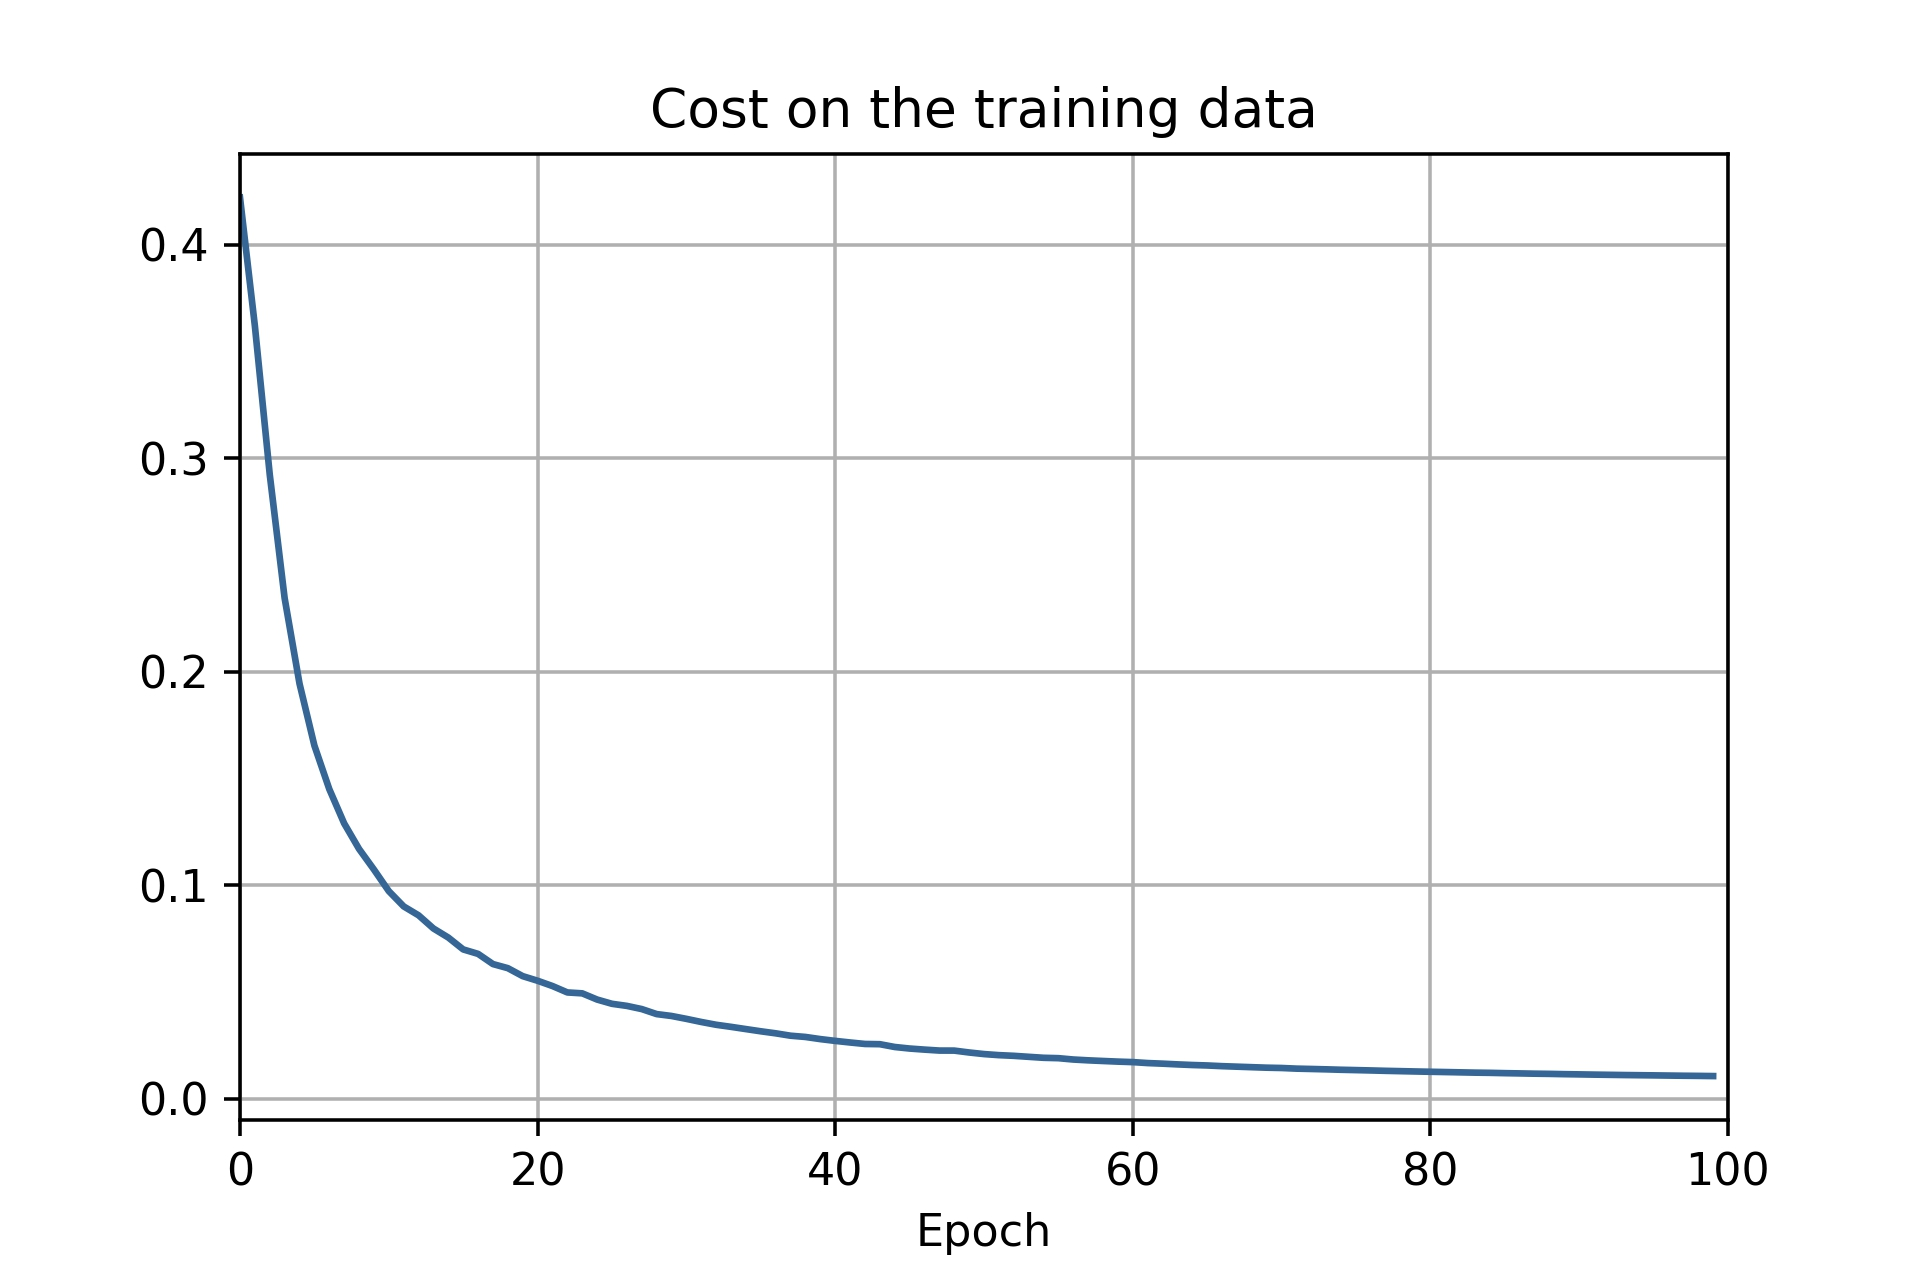
\includegraphics[scale=0.6]{"Part 3 - Learning Systems/Supervised Learning/Deep Learning/images/figure114.jpg"}
    \caption{Cost curve in training with 100 epochs and 1000 images.}
    \label{fig:figure114}
\end{figure}

At the end of the training, both networks had errors in the same order of magnitude, but the ability to recognize numbers is quite different between the two. This difference can be seen when comparing the accuracy graphs (Figures \ref{fig:figure115} and \ref{fig:figure116}) considering both training and validation data. The result of training with the entire dataset shows that the accuracy of the network for the validation data is very close to the result for the training values, a difference of 1\% . As for the situation that used only 1000 training data, the accuracy curves for the validation and training data are further apart, presenting a difference close to 14\%.

\begin{figure}
    \centering
    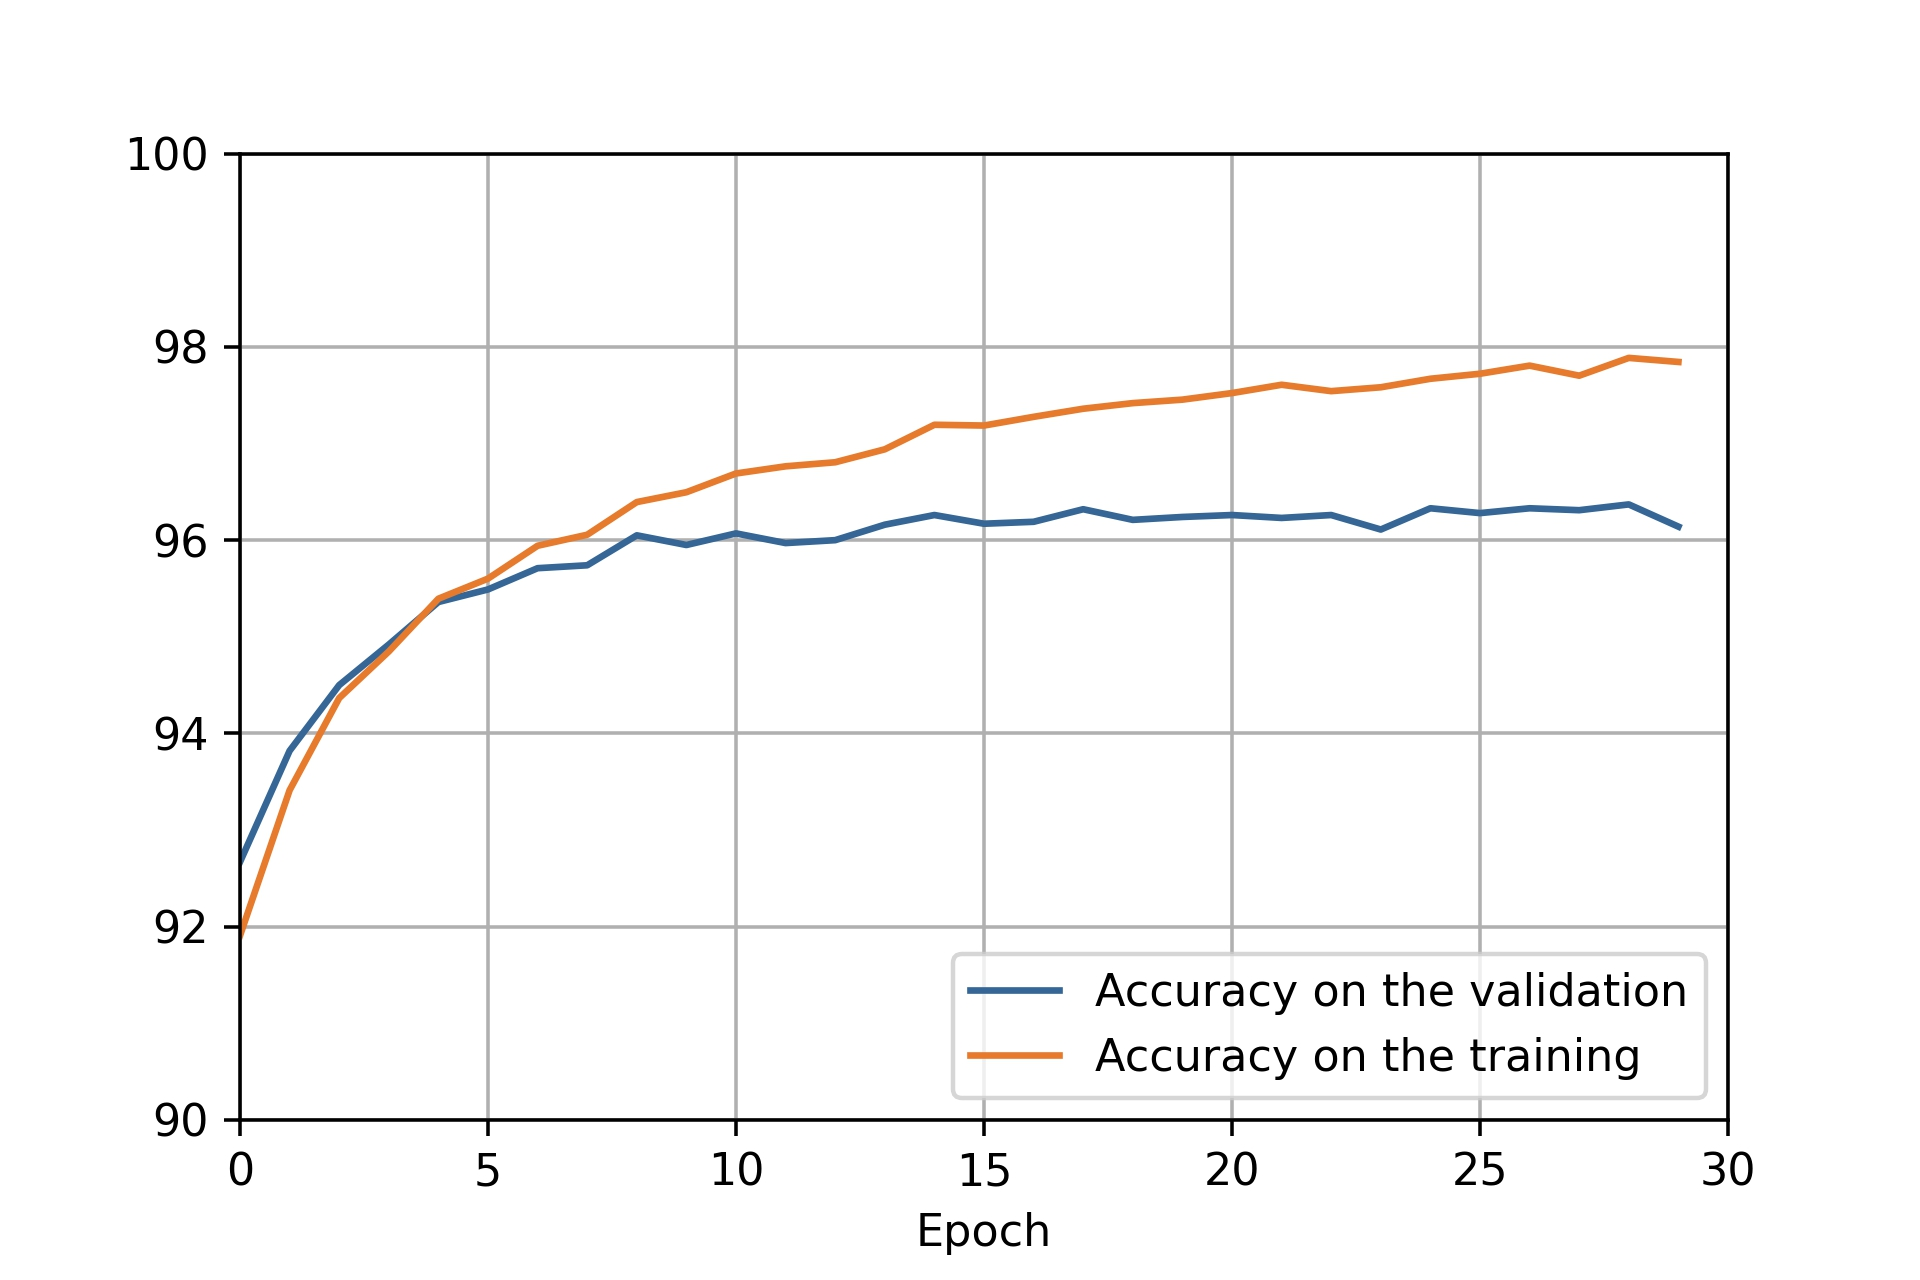
\includegraphics[scale=0.6]{"Part 3 - Learning Systems/Supervised Learning/Deep Learning/images/figure115.jpg"}
    \caption{Accuracy curves for a network trained with epochs 30 and 1000 images.}
    \label{fig:figure115}
\end{figure}

\begin{figure}
    \centering
    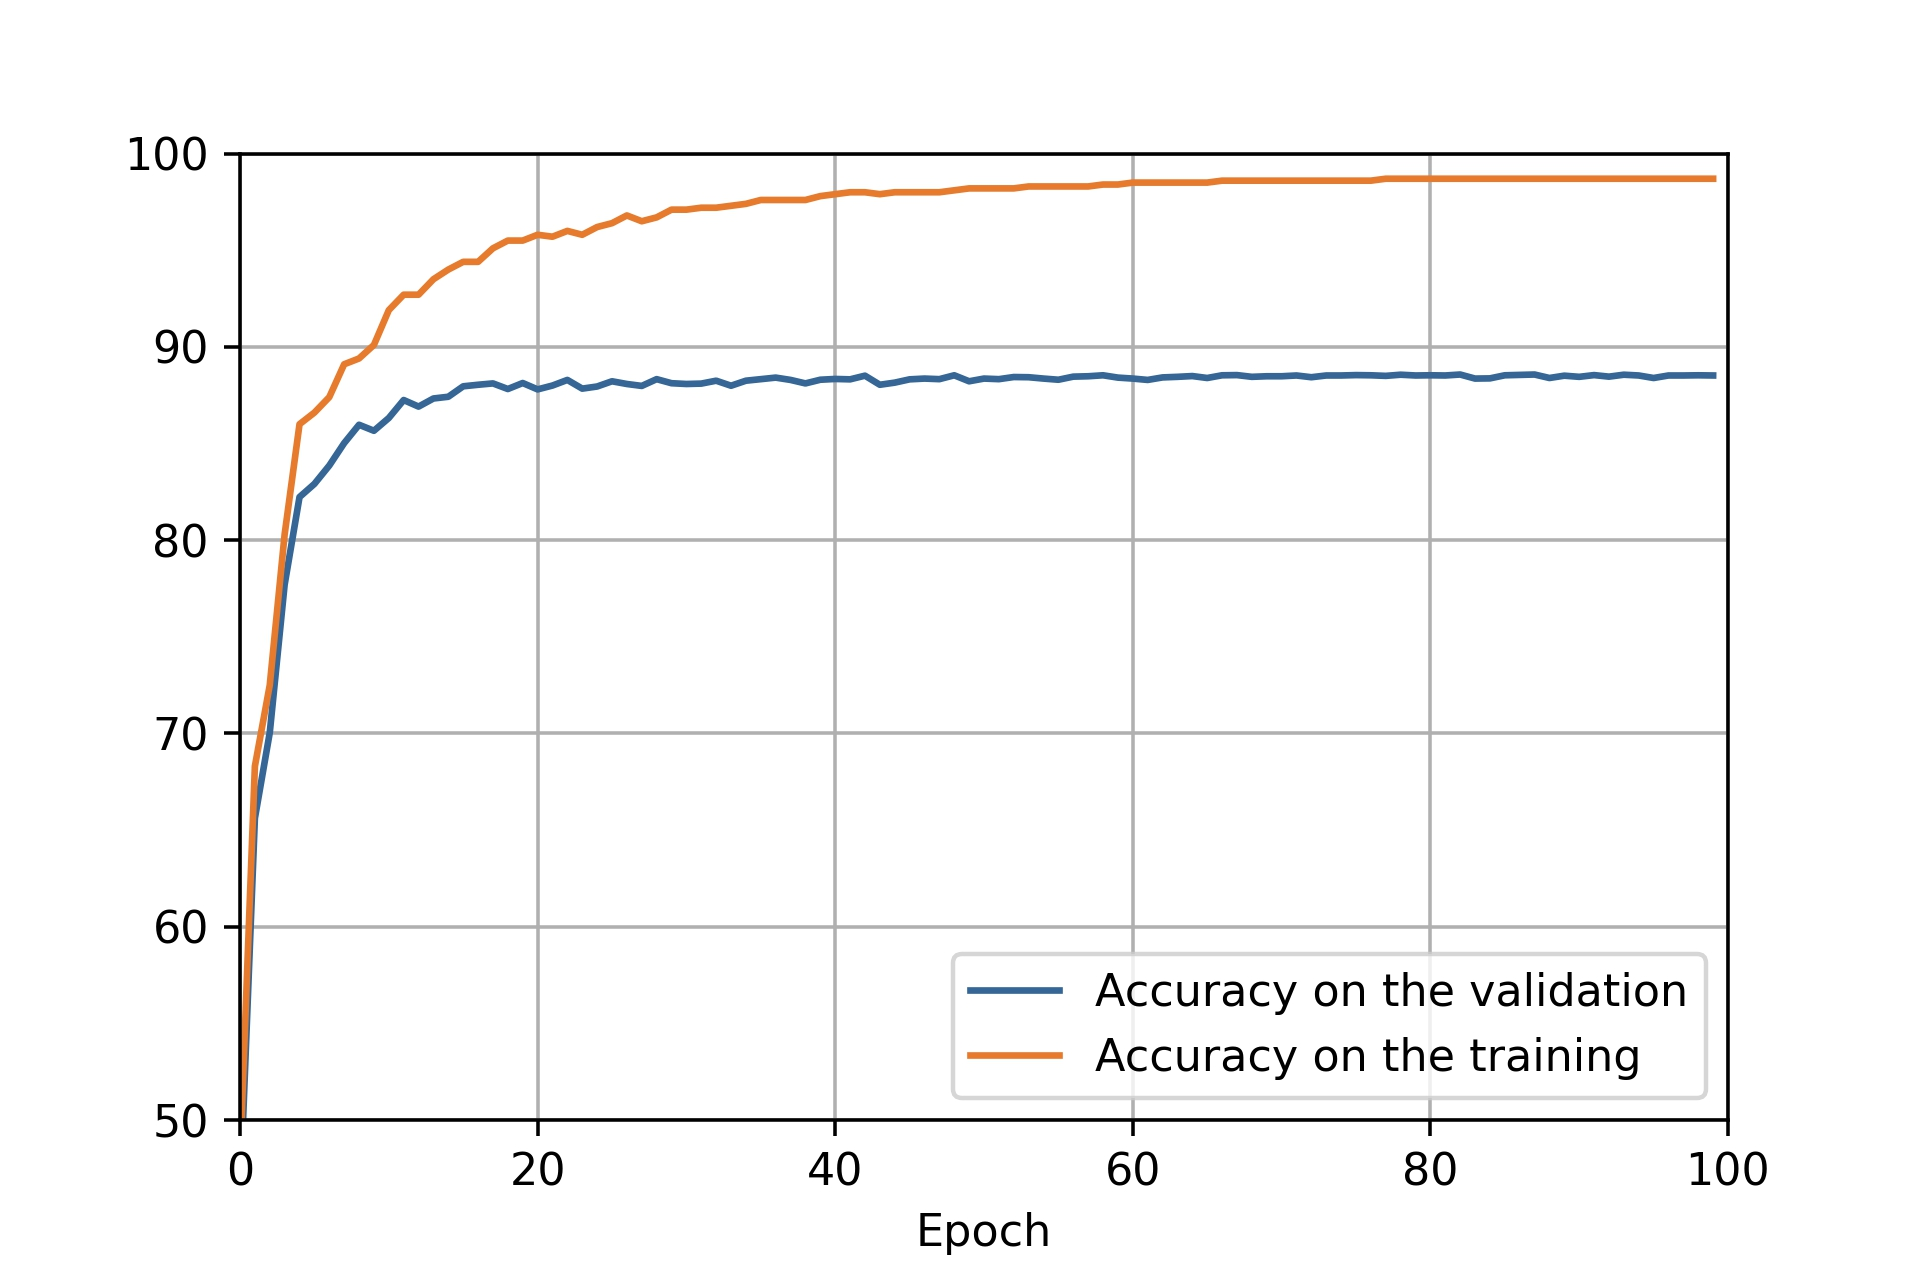
\includegraphics[scale=0.6]{"Part 3 - Learning Systems/Supervised Learning/Deep Learning/images/figure116.jpg"}
    \caption{Cost curve in training with 100 epochs and 1000 images.}
    \label{fig:figure116}
\end{figure}

By observing only the error curve, it is assumed that the network is learning until the end of the training, as the error continues to decrease. However, when analyzing the accuracy curves, it is identified that the accuracy determined by the validation data increases rapidly up to a certain time, close to 40 in the second case, and then becomes stagnant. Thus, after the 40th epoch, the network is no longer learning to generalize to the validation data, overfitting is occurring, that is, the training is not improving the network's capacity. Even though training accuracy is increasing after this time, it may be that the network is just memorizing training data, as it is no longer just sticking to the general information needed to recognize the numbers in general \cite{nielsen2015}.

The most common cases of overfitting occur when the number of training data is very low, as in this second case with only 1000 images. In this situation, the network has few examples to extract general information, often needing to increase the number of training times in order to reach a minimum performance. The greater the number of epochs, the more evident the overfiting effect may be, so it is recommended to observe when the validation accuracy starts to stagnate and get too far from the training curve \cite{nielsen2015}.

Observing the behavior of the validation accuracy is one of the methods to define how long the network should be trained, that is, the number of epochs. Validation data helps in testing different configurations of network hyperparameters such as training times, learning rate and number of nodes. Only after defining these parameters and training the network is it recommended to use the test data to really verify the accuracy of the network, using data that it has not yet had contact with \cite{nielsen2015}. A test with unknown data makes it possible to verify if the network parameters can be applied in more general cases or if they fit only in particularities of the trained data. For this reason, in most cases data is divided into three sets - training, validation and testing.